\justifying
\textbf{Цель работы:}
Научиться решать начальную задачу Коши для линейного ОДУ первого порядка.

\textbf{Задание:}
Исследовать численные решения начальной задачи Коши для линейного ОДУ первого порядка методом Рунге-Кутта четвертого порядка и многошаговым методом Адамса-Бэшфорта-Молтона. Исследовать абсолютную и относительную погрешности вычислений для случая
\begin{equation}\label{eq1}
    y' = y, \quad y(0) = 0, \quad x \in [0, 5]
\end{equation}
и
\begin{equation}\label{eq2}
    y' = -y, \quad y(0) = 1, \quad x \in [0, 5].
\end{equation}

\textbf{Ход работы:}

Уравнение в общем виде записывается как
\begin{equation}
    \frac{dy}{dx} = f(x,y),
\end{equation}
где
\begin{equation}
    f(x,y) = \pm y.
\end{equation}

Тогда метод Рунге-Кутта можно построить по следующим формулам:
\begin{equation}
\begin{cases}
    y_{n+1}=y_n+\frac{1}{6}(k_1+2k_2+2k_3+k_4), \\
    k_1=hf(x_n,y_n), \quad k_2=hf(x_n+\frac{1}{2} h, y_n+\frac{1}{2} k_1),\\
    k_3=hf(x_n+\frac{1}{2}h,y_n+\frac{1}{2}k_2), \quad k_4=hf(x_n+h,y_n+k_3)
\end{cases}
\end{equation}

Многошаговый метод Адамса-Бэшфорта-Молтона строится по формуле:
\begin{equation}
    y_{n+1}=y_n+\frac{h}{720}[1901f_{n}-2774f_{n-1}+2616f_{n-2}-1274f_{n-3}+251f_{n-4}].
\end{equation}
\newpage
Результаты реализации указанных методов для уравнений~(\ref{eq1}-\ref{eq2}) приведены ниже.
\begin{figure}[ht!]
    \centering
    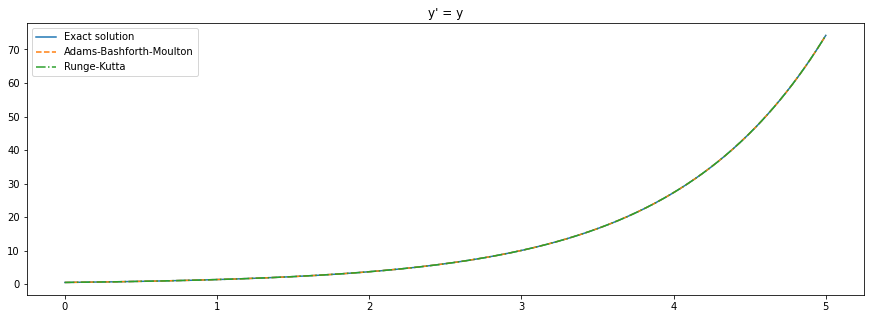
\includegraphics[width=\linewidth]{Figures/res1.png}
    \caption{Решение уравнения~(\ref{eq1}), полученное с помощью точного, Рунге-Кутта и Адамаса-Бэшфорта-Молтона}
    \label{fig:my_label}
\end{figure}

Из рисунка видно, что решения, полученные точно и с помощью итерационных методов Рунге-Кутта и Адамса-Бэшфорта-Молтона в общем совпадают. Для более детальной оценки решений, посмотрим на абсолютную и относительную погрешности вычислений, приведенные на Рисунке~\ref{fig:errors1}.
\newpage
\begin{figure}
    \centering
    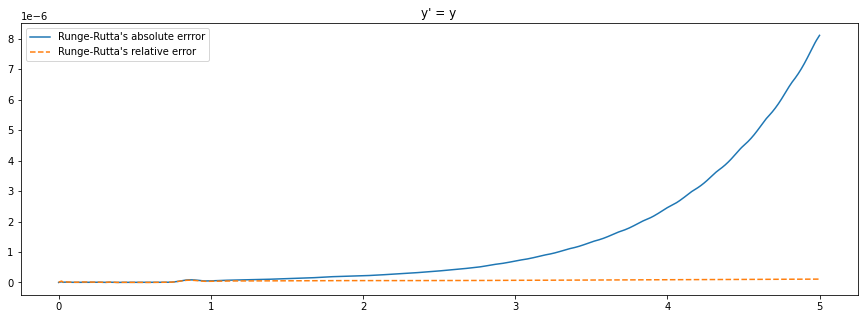
\includegraphics[width=\linewidth]{Figures/rk1.png}
    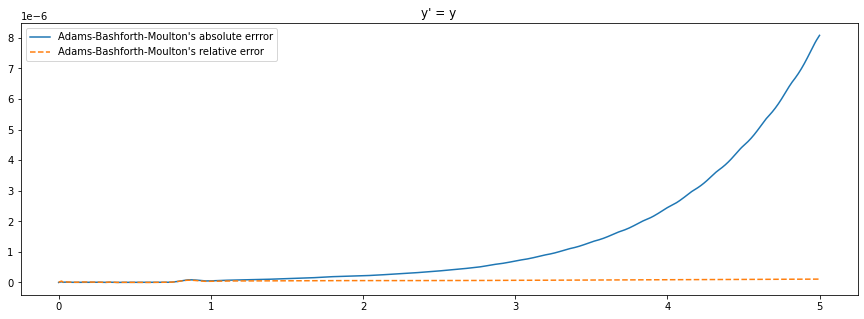
\includegraphics[width=\linewidth]{Figures/bm1.png}
    \caption{Графики абсолютной и относительной ошибок для точного и приближенного решений уравнения~(\ref{eq1}). Приближенное решение было получено с помощью методов Рунге-Кутта и Адамса-Бэшфорта-Молтона}
    \label{fig:errors1}
\end{figure}

Из рисунков видно, что абсолютная ошибка вычислений накапливается с ростом независимой переменной. Можно сделать вывод, что при значительных приростах независимой переменной численное решение методома Рунге-Кутта и Адамса-Бэшфорта-Молтона дифференциального уравнения первого порядка будет значительно отличаться от точного решения.
\newpage
\begin{figure}
    \centering
    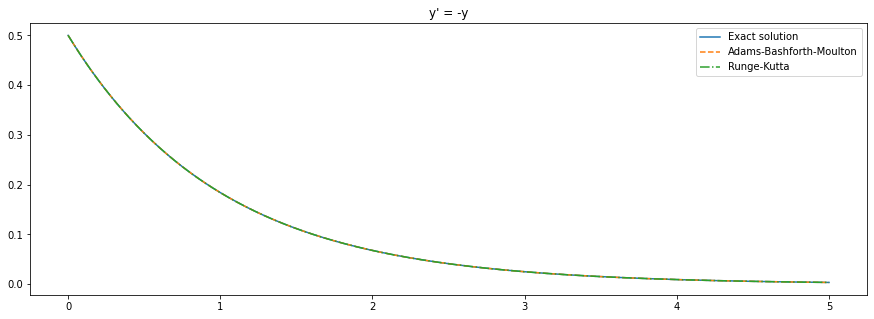
\includegraphics[width=\linewidth]{Figures/res2.png}
    \caption{Решение уравнения~(\ref{eq2}), полученное с помощью точного, Рунге-Кутта и Адамаса-Бэшфорта-Молтона}
    \label{fig:my_label}
\end{figure}

Из рисунка видно, что решения, полученные точно и с помощью итерационных методов Рунге-Кутта и Адамса-Бэшфорта-Молтона в общем совпадают. Для более детальной оценки решений, посмотрим на абсолютную и относительную погрешности вычислений, приведенные на Рисунке~\ref{fig:errors2}.
\newpage
\begin{figure}
    \centering
    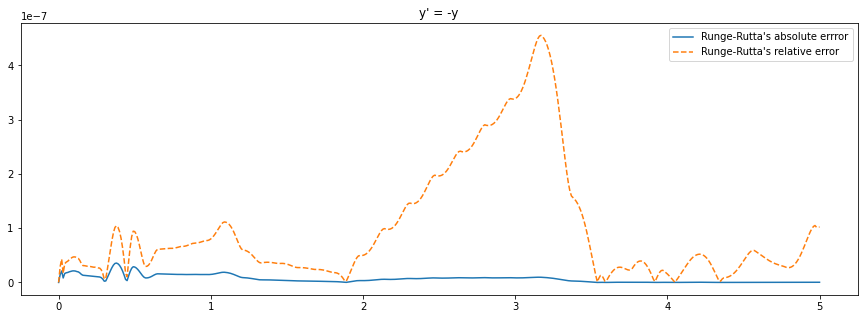
\includegraphics[width=\linewidth]{Figures/rk2.png}
    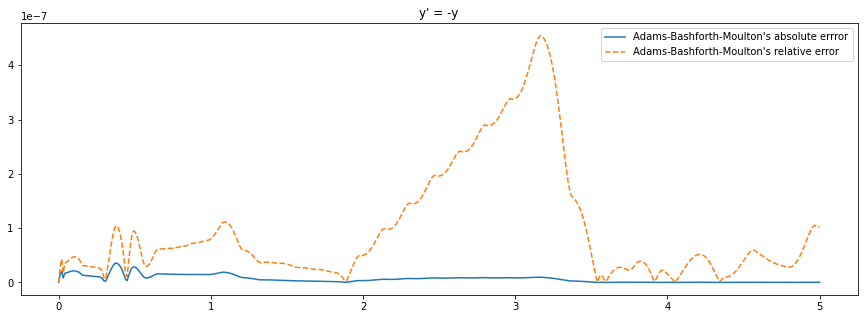
\includegraphics[width=\linewidth]{Figures/bm2.png}
    \caption{Графики абсолютной и относительной ошибок для точного и приближенного решений уравнения~(\ref{eq2}). Приближенное решение было получено с помощью методов Рунге-Кутта и Адамса-Бэшфорта-Молтона}
    \label{fig:errors2}
\end{figure}

Из рисунков видно, что относительная ошибка вычислений осциллирует с периодическим ростом при увеличивающейся независимой переменной. Можно сделать вывод, что местами численное решение методома Рунге-Кутта и Адамса-Бэшфорта-Молтона дифференциального уравнения первого порядка будет отличаться от точного решения. Однако, абсолютная погрешность остается практически равной нулю на всем отрезке $[0, 5]$.

\textbf{Выводы:}

В настоящей лабораторной работе были исследованы численные решения начальной задачи Коши для линейного ОДУ первого порядка методом Рунге-Кутта четвертого порядка и многошаговым методом Адамса-Бэшфорта-Молтона. Вычисления показали, что точное и приближенные решения совпадают на всем отрезке независимой переменной. Также были исследованы абсолютная и относительная погрешности вычислений для разных уравнений. Получилось, что для уравнения~(\ref{eq1}) в пределах отрезка $[0, 5]$ абсолютная погрешность возрастает с увеличением $x$. Для уравнения~(\ref{eq2}) абсолютная погрешность практически всегда остается равной нулю.